\documentclass[12pt]{article}
\usepackage{geometry}
\usepackage[hidelinks]{hyperref}
\usepackage{graphicx}
\usepackage{url}
\geometry{letterpaper,scale=0.85}
\title{\textbf{Project 1 process:\\Solved/confusing problems}}
\date{\textbf{\today}}

\begin{document}
	\maketitle
\tableofcontents
\newpage
	\thispagestyle{empty}
	\section{\textbf{Done so far}}
	Read the data \underline{polls\_us\_election\_2016.csv}\\
	Summary data
	\begin{figure}[h]
		\centering
		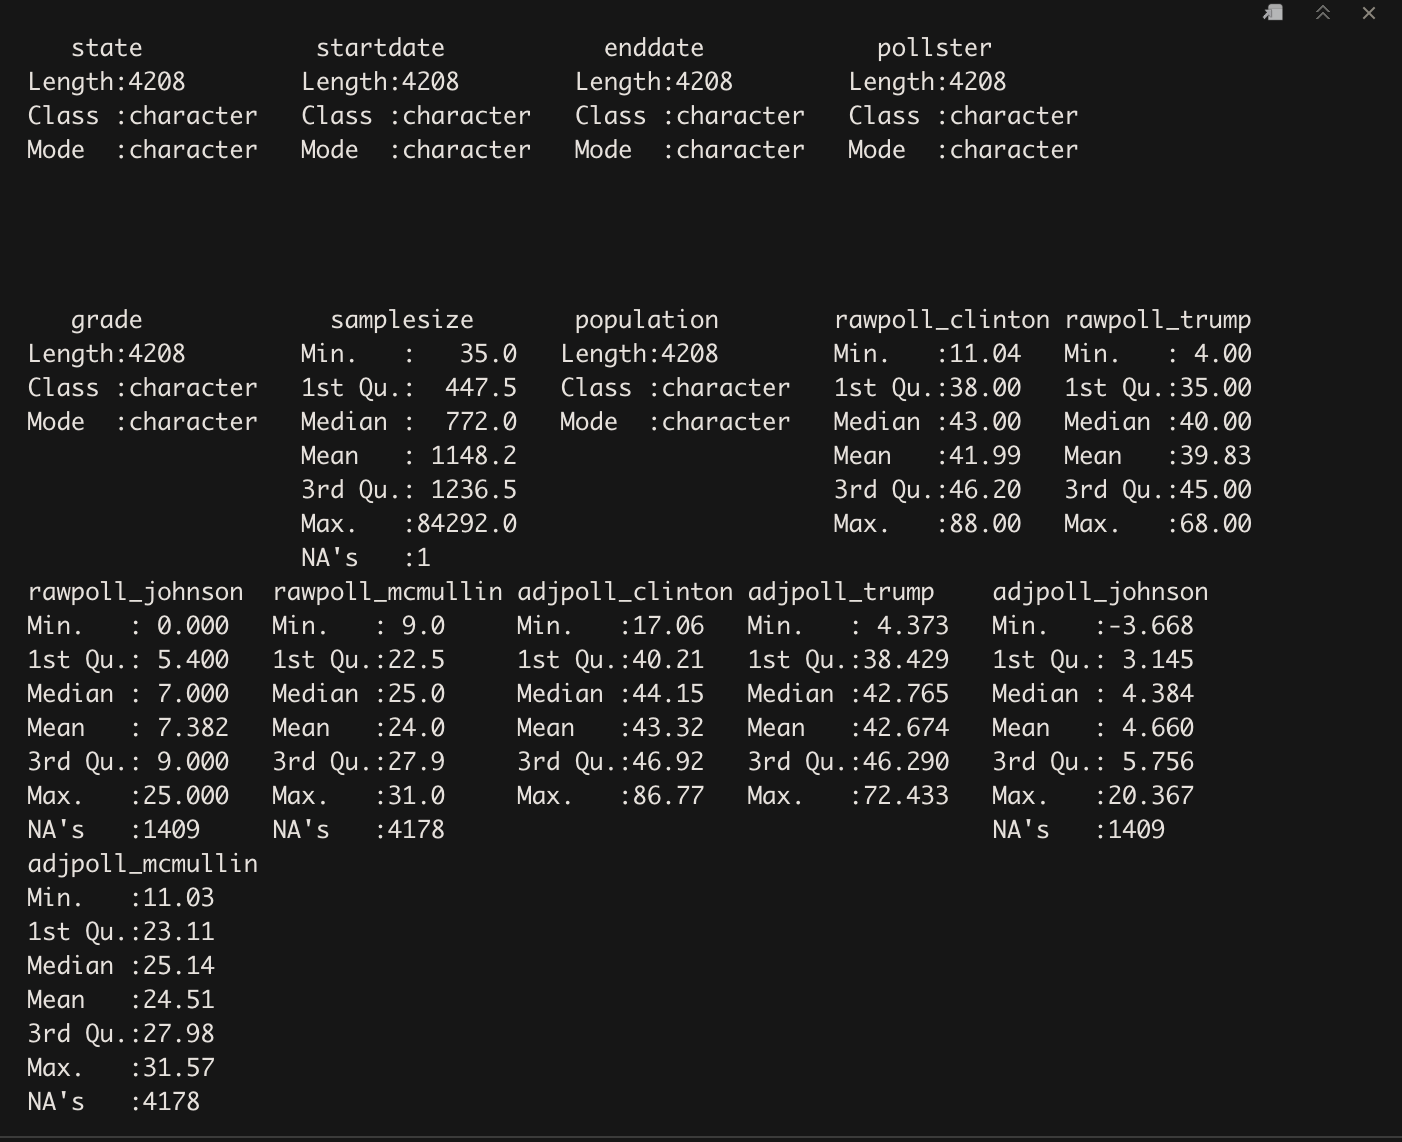
\includegraphics[width=1\textwidth]{summary.png} 
		\caption{Summary of polls\_us\_election\_2016.csv}
		\label{figure 1}
	\end{figure}
	\subsection{Explore variables}
	
	\begin{tabular}{|c|c|c|c|c|}
		\hline
		Variables & Size & Numbers of unique & Number of missings & Comment\\
		\hline
		state & 4208 & 55 & 0 &  “U.S.” means national polls \\
		\hline
		startdate & 4208 & 352 & 0 & E: 2015.11.06  L: 2016.11.06 \\
		\hline
		enddate & 4208 & 345 & 0 & E: 2015.11.08  L: 2016.11.07 \\
		\hline
		pollster & 4208 & 196 & 0 & just pollster's name \\
		\hline
		grade & 4208 & 11 (including NA) & 429 & see pdf files for exact numbers\\
		\hline
		population & 4208 & 4 & 0 & exact numbers for each on pdf \\
		\hline
		rawpoll\_clinton & 4208 & 1312 & 0 & Percentage \\
		\hline
		rawpoll\_trump & 4208 & 1385 & 0 & Percentage \\
		\hline
		rawpoll\_johnson & 4208 & 585 & 1409 & Percentage \\
		\hline
		rawpoll\_mcmullin & 4208 & 17 & 4178 & Percentage \\
		\hline
		adjpoll\_clinton & 4208 & 4200 & 0 & Percentage adjusted by 538 \\
		\hline
		adjpoll\_trump & 4208 & 4204 & 0 & Percentage adjusted by 538 \\
		\hline
		adjpoll\_johnson & 4208 & 2211 & 1409 & Percentage adjusted by 538 \\
		\hline
		adjpoll\_mcmullin & 4208 & 31 & 4178 & Percentage adjusted by 538 \\
		\hline
	\end{tabular}
	        
	\subsection{data dictionary}
	\subsubsection{state}
	The name of the state where the election is held, “U.S.” means national polls.
	\subsubsection{startdate}
	Start data of poll.
	\subsubsection{enddate}
	End data of poll.
	\subsubsection{pollster}
	Organization name that conducts or analyzes opinion polls.
	\subsubsection{grade}
	Grade assigned by Fivethirtyeight (sometimes as 538, an American website that focuses on opinion poll) to pollster.\\
	"A letter grade from A+ to F that reflects the accuracy of a polling organization's polls and its predictive plus-minus score (a projection of how well we think a pollster's polls will do in the future). Pollsters with a small number of polls get a provisional rating (for example, A/B) rather than a precise letter grade“ (Cite from \url{ https://projects.fivethirtyeight.com/pollster-ratings/}).
	\subsubsection{samplesize}
	Sample size of polls for each pollster.
	\subsubsection{population}
	Type of population being polled.
	
	\begin{itemize}
		\item LV(likely Voters): \\population whose most likely to participate in 2016 election
		\item RV (Registered Voters): \\RV includes all eligible and registered voters, whether or not they end up voting.
		\item A (Adults): \\Refers to all persons of legal voting age.
		\item V (Voters): \\Persons who has voted in an election.
	\end{itemize}
	
	\subsubsection{rawpoll\_clinton}
	Percentage for Hillary Clinton.
	\subsubsection{rawpoll\_trump}
	Percentage for Donald Trump.
	\subsubsection{rawpoll\_johnson}
	Percentage for Gary Johnson.
	\subsubsection{rawpoll\_mcmullin}
	Percentage for Evan Mcmullin.
	\subsubsection{adjpoll\_clinton}
	Fivethirtyeight adjusted percentage for Hillary Clinton.
	\subsubsection{adjpoll\_trump}
	Fivethirtyeight adjusted percentage for Donald Trump.
	\subsubsection{adjpoll\_johnson}
	Fivethirtyeight adjusted percentage for Gary Johnson.
	\subsubsection{adjpoll\_mcmullin}
	Fivethirtyeight adjusted percentage for Evan Mcmullin.
	\section{\textbf{Problems}}
	\section{\textbf{Plans}}
	
	
\end{document}